\section{Process Class Reference}
\label{classProcess}\index{Process@{Process}}
Inheritance diagram for Process:\begin{figure}[H]
\begin{center}
\leavevmode
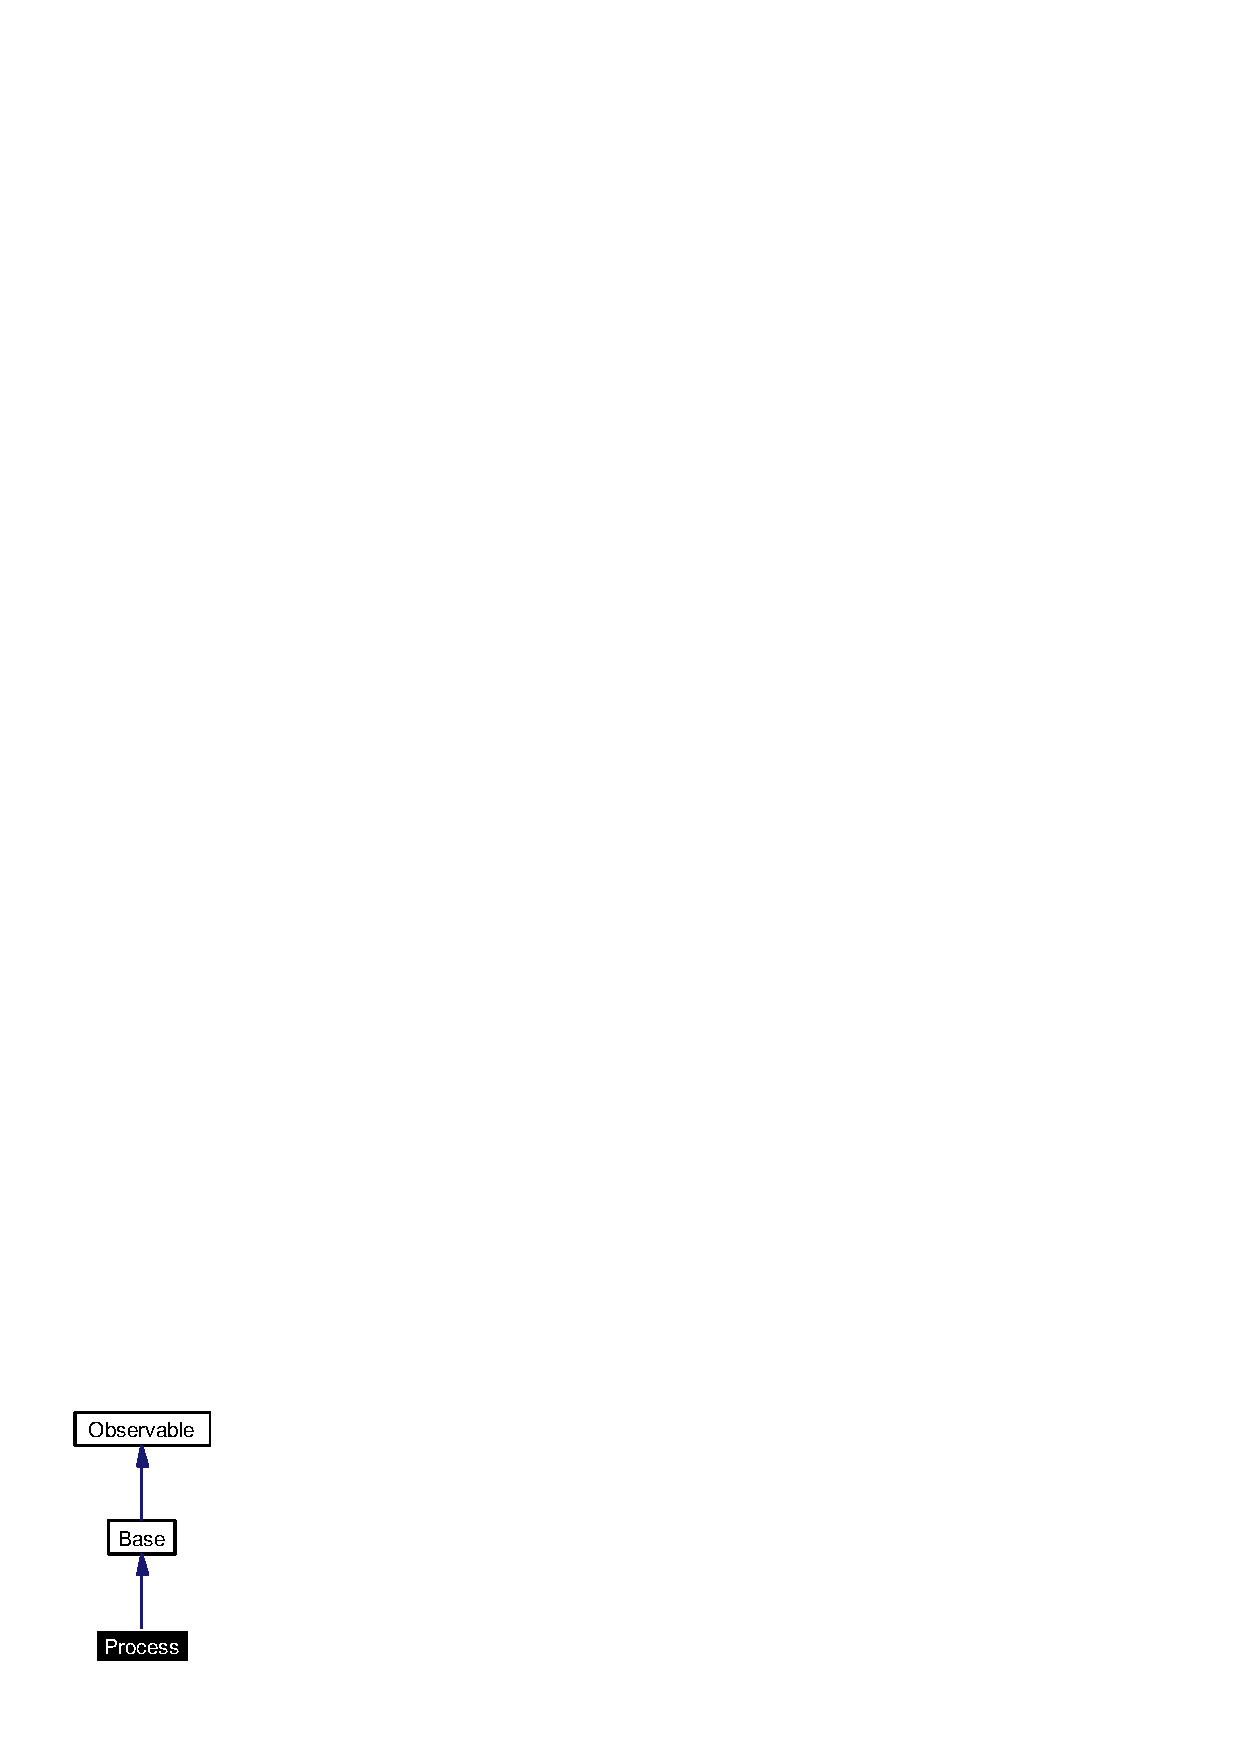
\includegraphics[width=50pt]{classProcess__inherit__graph}
\end{center}
\end{figure}
Collaboration diagram for Process:\begin{figure}[H]
\begin{center}
\leavevmode
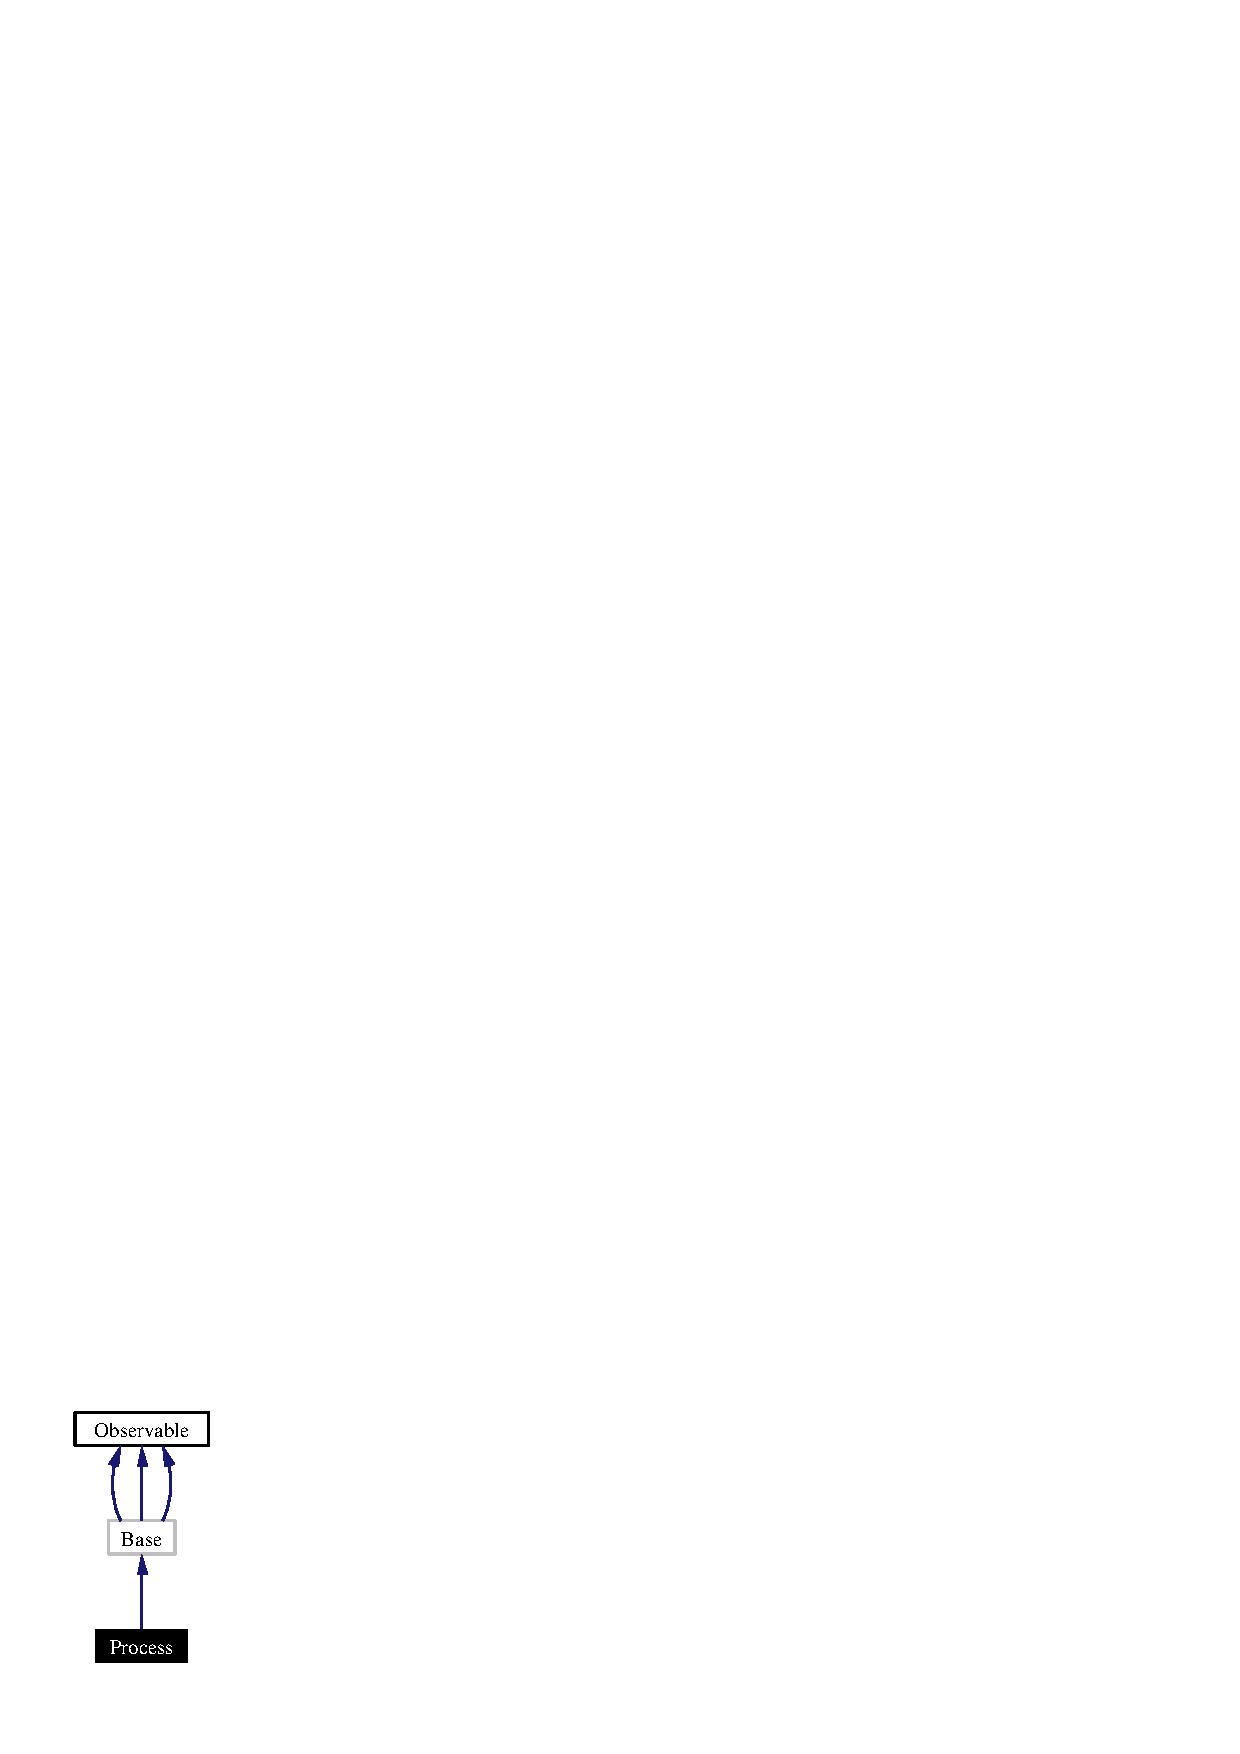
\includegraphics[width=50pt]{classProcess__coll__graph}
\end{center}
\end{figure}
\subsection*{Public Member Functions}
\begin{CompactItemize}
\item 
\index{Process@{Process}!Process@{Process}}\index{Process@{Process}!Process@{Process}}
{\bf Process} (\$db)\label{classProcess_a0}

\item 
{\bf get\-Process} (\$p\-Id)
\item 
{\bf get\-Normalized\-Name} ()
\item 
{\bf get\-Name} ()
\item 
{\bf get\-Version} ()
\end{CompactItemize}
\subsection*{Public Attributes}
\begin{CompactItemize}
\item 
\index{name@{name}!Process@{Process}}\index{Process@{Process}!name@{name}}
{\bf name}\label{classProcess_m0}

\item 
\index{description@{description}!Process@{Process}}\index{Process@{Process}!description@{description}}
{\bf description}\label{classProcess_m1}

\item 
\index{version@{version}!Process@{Process}}\index{Process@{Process}!version@{version}}
{\bf version}\label{classProcess_m2}

\item 
\index{normalizedName@{normalizedName}!Process@{Process}}\index{Process@{Process}!normalizedName@{normalizedName}}
{\bf normalized\-Name}\label{classProcess_m3}

\end{CompactItemize}


\subsection{Detailed Description}
This class representes the process that is being executed when an activity is executed. You can access this class methods using \$process from any activity. No need to instantiate a new object. 



Definition at line 9 of file Process.php.

\subsection{Member Function Documentation}
\index{Process@{Process}!getName@{getName}}
\index{getName@{getName}!Process@{Process}}
\subsubsection{\setlength{\rightskip}{0pt plus 5cm}Process::get\-Name ()}\label{classProcess_a3}


Gets the process name

Definition at line 46 of file Process.php.\index{Process@{Process}!getNormalizedName@{getNormalizedName}}
\index{getNormalizedName@{getNormalizedName}!Process@{Process}}
\subsubsection{\setlength{\rightskip}{0pt plus 5cm}Process::get\-Normalized\-Name ()}\label{classProcess_a2}


Gets the normalized name of the process

Definition at line 38 of file Process.php.\index{Process@{Process}!getProcess@{getProcess}}
\index{getProcess@{getProcess}!Process@{Process}}
\subsubsection{\setlength{\rightskip}{0pt plus 5cm}Process::get\-Process (\$ {\em p\-Id})}\label{classProcess_a1}


Loads a process form the database

Definition at line 23 of file Process.php.\index{Process@{Process}!getVersion@{getVersion}}
\index{getVersion@{getVersion}!Process@{Process}}
\subsubsection{\setlength{\rightskip}{0pt plus 5cm}Process::get\-Version ()}\label{classProcess_a4}


Gets the process version

Definition at line 54 of file Process.php.

The documentation for this class was generated from the following file:\begin{CompactItemize}
\item 
Process.php\end{CompactItemize}
